% Options for packages loaded elsewhere
\PassOptionsToPackage{unicode}{hyperref}
\PassOptionsToPackage{hyphens}{url}
\PassOptionsToPackage{dvipsnames,svgnames,x11names}{xcolor}
%
\documentclass[
  a4paper,
]{book}

\usepackage{amsmath,amssymb}
\usepackage{iftex}
\ifPDFTeX
  \usepackage[T1]{fontenc}
  \usepackage[utf8]{inputenc}
  \usepackage{textcomp} % provide euro and other symbols
\else % if luatex or xetex
  \usepackage{unicode-math}
  \defaultfontfeatures{Scale=MatchLowercase}
  \defaultfontfeatures[\rmfamily]{Ligatures=TeX,Scale=1}
\fi
\usepackage{lmodern}
\ifPDFTeX\else  
    % xetex/luatex font selection
\fi
% Use upquote if available, for straight quotes in verbatim environments
\IfFileExists{upquote.sty}{\usepackage{upquote}}{}
\IfFileExists{microtype.sty}{% use microtype if available
  \usepackage[]{microtype}
  \UseMicrotypeSet[protrusion]{basicmath} % disable protrusion for tt fonts
}{}
\makeatletter
\@ifundefined{KOMAClassName}{% if non-KOMA class
  \IfFileExists{parskip.sty}{%
    \usepackage{parskip}
  }{% else
    \setlength{\parindent}{0pt}
    \setlength{\parskip}{6pt plus 2pt minus 1pt}}
}{% if KOMA class
  \KOMAoptions{parskip=half}}
\makeatother
\usepackage{xcolor}
\usepackage[paperwidth=8.27in,paperheight=11.69in,left=1.25in,textwidth=
5.25in,top=1.00in,textheight=8.25in]{geometry}
\setlength{\emergencystretch}{3em} % prevent overfull lines
\setcounter{secnumdepth}{5}
% Make \paragraph and \subparagraph free-standing
\ifx\paragraph\undefined\else
  \let\oldparagraph\paragraph
  \renewcommand{\paragraph}[1]{\oldparagraph{#1}\mbox{}}
\fi
\ifx\subparagraph\undefined\else
  \let\oldsubparagraph\subparagraph
  \renewcommand{\subparagraph}[1]{\oldsubparagraph{#1}\mbox{}}
\fi

\usepackage{color}
\usepackage{fancyvrb}
\newcommand{\VerbBar}{|}
\newcommand{\VERB}{\Verb[commandchars=\\\{\}]}
\DefineVerbatimEnvironment{Highlighting}{Verbatim}{commandchars=\\\{\}}
% Add ',fontsize=\small' for more characters per line
\usepackage{framed}
\definecolor{shadecolor}{RGB}{241,243,245}
\newenvironment{Shaded}{\begin{snugshade}}{\end{snugshade}}
\newcommand{\AlertTok}[1]{\textcolor[rgb]{0.68,0.00,0.00}{#1}}
\newcommand{\AnnotationTok}[1]{\textcolor[rgb]{0.37,0.37,0.37}{#1}}
\newcommand{\AttributeTok}[1]{\textcolor[rgb]{0.40,0.45,0.13}{#1}}
\newcommand{\BaseNTok}[1]{\textcolor[rgb]{0.68,0.00,0.00}{#1}}
\newcommand{\BuiltInTok}[1]{\textcolor[rgb]{0.00,0.23,0.31}{#1}}
\newcommand{\CharTok}[1]{\textcolor[rgb]{0.13,0.47,0.30}{#1}}
\newcommand{\CommentTok}[1]{\textcolor[rgb]{0.37,0.37,0.37}{#1}}
\newcommand{\CommentVarTok}[1]{\textcolor[rgb]{0.37,0.37,0.37}{\textit{#1}}}
\newcommand{\ConstantTok}[1]{\textcolor[rgb]{0.56,0.35,0.01}{#1}}
\newcommand{\ControlFlowTok}[1]{\textcolor[rgb]{0.00,0.23,0.31}{#1}}
\newcommand{\DataTypeTok}[1]{\textcolor[rgb]{0.68,0.00,0.00}{#1}}
\newcommand{\DecValTok}[1]{\textcolor[rgb]{0.68,0.00,0.00}{#1}}
\newcommand{\DocumentationTok}[1]{\textcolor[rgb]{0.37,0.37,0.37}{\textit{#1}}}
\newcommand{\ErrorTok}[1]{\textcolor[rgb]{0.68,0.00,0.00}{#1}}
\newcommand{\ExtensionTok}[1]{\textcolor[rgb]{0.00,0.23,0.31}{#1}}
\newcommand{\FloatTok}[1]{\textcolor[rgb]{0.68,0.00,0.00}{#1}}
\newcommand{\FunctionTok}[1]{\textcolor[rgb]{0.28,0.35,0.67}{#1}}
\newcommand{\ImportTok}[1]{\textcolor[rgb]{0.00,0.46,0.62}{#1}}
\newcommand{\InformationTok}[1]{\textcolor[rgb]{0.37,0.37,0.37}{#1}}
\newcommand{\KeywordTok}[1]{\textcolor[rgb]{0.00,0.23,0.31}{#1}}
\newcommand{\NormalTok}[1]{\textcolor[rgb]{0.00,0.23,0.31}{#1}}
\newcommand{\OperatorTok}[1]{\textcolor[rgb]{0.37,0.37,0.37}{#1}}
\newcommand{\OtherTok}[1]{\textcolor[rgb]{0.00,0.23,0.31}{#1}}
\newcommand{\PreprocessorTok}[1]{\textcolor[rgb]{0.68,0.00,0.00}{#1}}
\newcommand{\RegionMarkerTok}[1]{\textcolor[rgb]{0.00,0.23,0.31}{#1}}
\newcommand{\SpecialCharTok}[1]{\textcolor[rgb]{0.37,0.37,0.37}{#1}}
\newcommand{\SpecialStringTok}[1]{\textcolor[rgb]{0.13,0.47,0.30}{#1}}
\newcommand{\StringTok}[1]{\textcolor[rgb]{0.13,0.47,0.30}{#1}}
\newcommand{\VariableTok}[1]{\textcolor[rgb]{0.07,0.07,0.07}{#1}}
\newcommand{\VerbatimStringTok}[1]{\textcolor[rgb]{0.13,0.47,0.30}{#1}}
\newcommand{\WarningTok}[1]{\textcolor[rgb]{0.37,0.37,0.37}{\textit{#1}}}

\providecommand{\tightlist}{%
  \setlength{\itemsep}{0pt}\setlength{\parskip}{0pt}}\usepackage{longtable,booktabs,array}
\usepackage{calc} % for calculating minipage widths
% Correct order of tables after \paragraph or \subparagraph
\usepackage{etoolbox}
\makeatletter
\patchcmd\longtable{\par}{\if@noskipsec\mbox{}\fi\par}{}{}
\makeatother
% Allow footnotes in longtable head/foot
\IfFileExists{footnotehyper.sty}{\usepackage{footnotehyper}}{\usepackage{footnote}}
\makesavenoteenv{longtable}
\usepackage{graphicx}
\makeatletter
\def\maxwidth{\ifdim\Gin@nat@width>\linewidth\linewidth\else\Gin@nat@width\fi}
\def\maxheight{\ifdim\Gin@nat@height>\textheight\textheight\else\Gin@nat@height\fi}
\makeatother
% Scale images if necessary, so that they will not overflow the page
% margins by default, and it is still possible to overwrite the defaults
% using explicit options in \includegraphics[width, height, ...]{}
\setkeys{Gin}{width=\maxwidth,height=\maxheight,keepaspectratio}
% Set default figure placement to htbp
\makeatletter
\def\fps@figure{htbp}
\makeatother
% definitions for citeproc citations
\NewDocumentCommand\citeproctext{}{}
\NewDocumentCommand\citeproc{mm}{%
  \begingroup\def\citeproctext{#2}\cite{#1}\endgroup}
\makeatletter
 % allow citations to break across lines
 \let\@cite@ofmt\@firstofone
 % avoid brackets around text for \cite:
 \def\@biblabel#1{}
 \def\@cite#1#2{{#1\if@tempswa , #2\fi}}
\makeatother
\newlength{\cslhangindent}
\setlength{\cslhangindent}{1.5em}
\newlength{\csllabelwidth}
\setlength{\csllabelwidth}{3em}
\newenvironment{CSLReferences}[2] % #1 hanging-indent, #2 entry-spacing
 {\begin{list}{}{%
  \setlength{\itemindent}{0pt}
  \setlength{\leftmargin}{0pt}
  \setlength{\parsep}{0pt}
  % turn on hanging indent if param 1 is 1
  \ifodd #1
   \setlength{\leftmargin}{\cslhangindent}
   \setlength{\itemindent}{-1\cslhangindent}
  \fi
  % set entry spacing
  \setlength{\itemsep}{#2\baselineskip}}}
 {\end{list}}
\usepackage{calc}
\newcommand{\CSLBlock}[1]{\hfill\break\parbox[t]{\linewidth}{\strut\ignorespaces#1\strut}}
\newcommand{\CSLLeftMargin}[1]{\parbox[t]{\csllabelwidth}{\strut#1\strut}}
\newcommand{\CSLRightInline}[1]{\parbox[t]{\linewidth - \csllabelwidth}{\strut#1\strut}}
\newcommand{\CSLIndent}[1]{\hspace{\cslhangindent}#1}

\usepackage{makeidx}
\makeindex
\usepackage{titling}
\usepackage{pdfpages}
\usepackage{atbegshi}% http://ctan.org/pkg/atbegshi
\let\oldmaketitle\maketitle
\AtBeginDocument{\let\maketitle\relax}
\AtBeginDocument{\AtBeginShipoutNext{\AtBeginShipoutDiscard}} % Discard next blank page

\makeatletter
\@ifpackageloaded{tcolorbox}{}{\usepackage[skins,breakable]{tcolorbox}}
\@ifpackageloaded{fontawesome5}{}{\usepackage{fontawesome5}}
\definecolor{quarto-callout-color}{HTML}{909090}
\definecolor{quarto-callout-note-color}{HTML}{0758E5}
\definecolor{quarto-callout-important-color}{HTML}{CC1914}
\definecolor{quarto-callout-warning-color}{HTML}{EB9113}
\definecolor{quarto-callout-tip-color}{HTML}{00A047}
\definecolor{quarto-callout-caution-color}{HTML}{FC5300}
\definecolor{quarto-callout-color-frame}{HTML}{acacac}
\definecolor{quarto-callout-note-color-frame}{HTML}{4582ec}
\definecolor{quarto-callout-important-color-frame}{HTML}{d9534f}
\definecolor{quarto-callout-warning-color-frame}{HTML}{f0ad4e}
\definecolor{quarto-callout-tip-color-frame}{HTML}{02b875}
\definecolor{quarto-callout-caution-color-frame}{HTML}{fd7e14}
\makeatother
\makeatletter
\@ifpackageloaded{bookmark}{}{\usepackage{bookmark}}
\makeatother
\makeatletter
\@ifpackageloaded{caption}{}{\usepackage{caption}}
\AtBeginDocument{%
\ifdefined\contentsname
  \renewcommand*\contentsname{Índice}
\else
  \newcommand\contentsname{Índice}
\fi
\ifdefined\listfigurename
  \renewcommand*\listfigurename{Lista de Figuras}
\else
  \newcommand\listfigurename{Lista de Figuras}
\fi
\ifdefined\listtablename
  \renewcommand*\listtablename{Lista de Tabelas}
\else
  \newcommand\listtablename{Lista de Tabelas}
\fi
\ifdefined\figurename
  \renewcommand*\figurename{Figura}
\else
  \newcommand\figurename{Figura}
\fi
\ifdefined\tablename
  \renewcommand*\tablename{Tabela}
\else
  \newcommand\tablename{Tabela}
\fi
}
\@ifpackageloaded{float}{}{\usepackage{float}}
\floatstyle{ruled}
\@ifundefined{c@chapter}{\newfloat{codelisting}{h}{lop}}{\newfloat{codelisting}{h}{lop}[chapter]}
\floatname{codelisting}{Listagem}
\newcommand*\listoflistings{\listof{codelisting}{Lista de Listagens}}
\makeatother
\makeatletter
\makeatother
\makeatletter
\@ifpackageloaded{caption}{}{\usepackage{caption}}
\@ifpackageloaded{subcaption}{}{\usepackage{subcaption}}
\makeatother
\newcounter{quartocallouttipno}
\newcommand{\quartocallouttip}[1]{\refstepcounter{quartocallouttipno}\label{#1}}
\ifLuaTeX
\usepackage[bidi=basic]{babel}
\else
\usepackage[bidi=default]{babel}
\fi
\babelprovide[main,import]{portuguese}
% get rid of language-specific shorthands (see #6817):
\let\LanguageShortHands\languageshorthands
\def\languageshorthands#1{}
\ifLuaTeX
  \usepackage{selnolig}  % disable illegal ligatures
\fi
\usepackage{bookmark}

\IfFileExists{xurl.sty}{\usepackage{xurl}}{} % add URL line breaks if available
\urlstyle{same} % disable monospaced font for URLs
\hypersetup{
  pdftitle={Finanças Corporativas de Curto Prazo},
  pdfauthor={Pablo Rogers},
  pdflang={pt},
  colorlinks=true,
  linkcolor={Maroon},
  filecolor={Maroon},
  citecolor={Blue},
  urlcolor={Blue},
  pdfcreator={LaTeX via pandoc}}

\title{Finanças Corporativas de Curto Prazo}
\author{Pablo Rogers}
\date{5 de junho de 2025}

\begin{document}
\frontmatter
\maketitle

\begin{center}
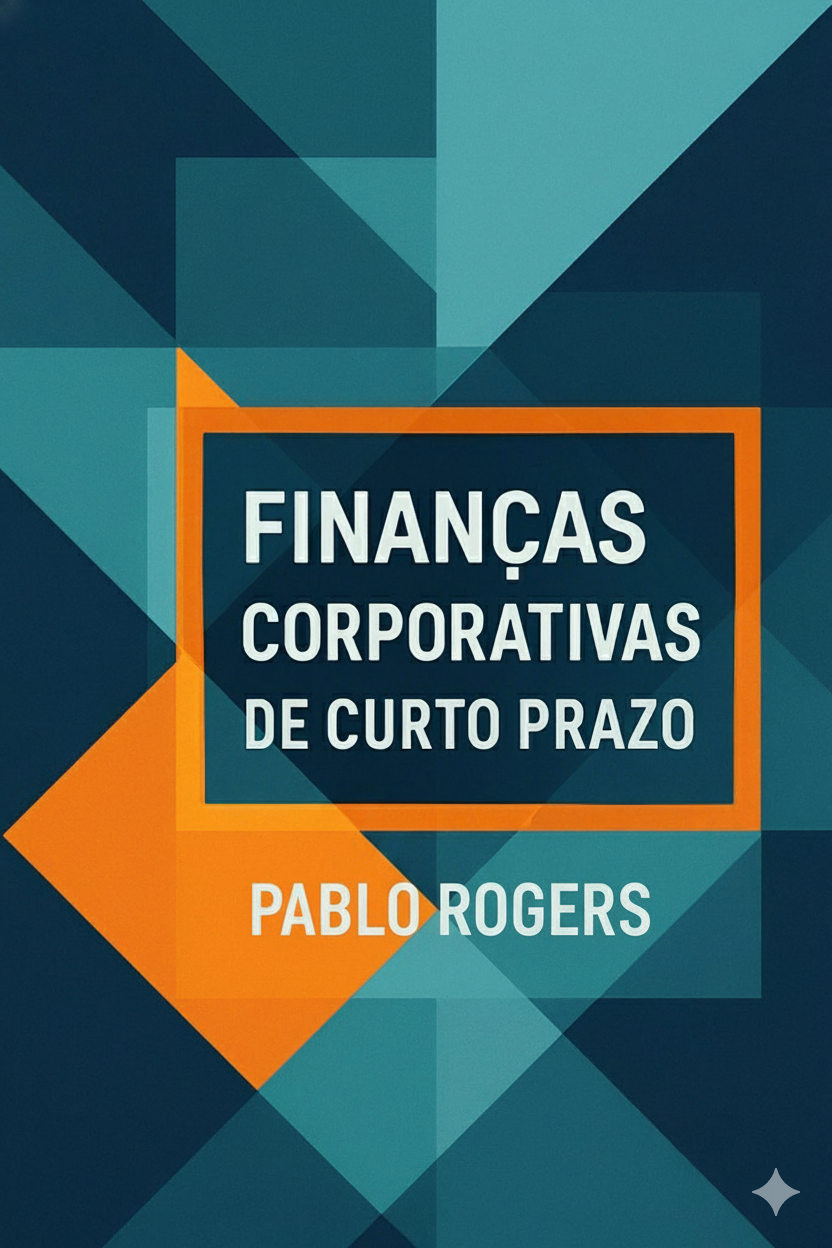
\includepdf[fitpaper=true,pages=-]{img/cover-book}
\end{center}
\let\maketitle\oldmaketitle
\maketitle
\AtBeginShipoutNext{\AtBeginShipoutDiscard}
\mainmatter
%\pagestyle{plain}

\renewcommand*\contentsname{Índice}
{
\hypersetup{linkcolor=}
\setcounter{tocdepth}{2}
\tableofcontents
}
\mainmatter
\bookmarksetup{startatroot}

\chapter*{O Curso 🏢}\label{sec-home}
\addcontentsline{toc}{chapter}{O Curso 🏢}

\markboth{O Curso 🏢}{O Curso 🏢}

Página da disciplina \textbf{``Finanças Corporativas I''} do curso de
\href{https://www.facic.ufu.br/}{Ciência Contábeis} da
\href{https://ufu.br/}{Universidade Federal de Uberlândia} . Aqui você
encontrará informações sobre o programa do curso, materiais para seu
acompanhamento e sugestões de leituras sobre o \textbf{Finanças
Corporativas de Curto Prazo} (artigos, notas de aulas, blogs, vídeos,
etc.).

\section*{Sobre o professor}\label{sec-instrutor}

\markright{Sobre o professor}

A disciplina é ministrada e mantida nesse hub por mim, Pablo Rogers,
doutor em administração pela Universidade de São Paulo (FEA/USP) e
professor de finanças e métodos quantitativos desde 2005. Em meu
\href{https://phdpablo.com/}{site pessoal} você encontra mais detalhes
sobre minhas formações, competências, trajetória e projetos.

\section*{Objetivos}\label{sec-about}

\markright{Objetivos}

O curso tem como objetivo apresentar os principais conceitos e práticas
de finanças corporativas de curto prazo\ldots{}

\section*{Ementa}\label{sec-ementa}

\markright{Ementa}

A ementa oficial da disciplina encontra-se
\href{https://www.facic.ufu.br/system/files/conteudo/28fagen39532_financas_corporativas_i.pdf}{aqui}.

\section*{Metodologia}\label{sec-method}

\markright{Metodologia}

O material do curso organizado nesse repositório refere-se ao roteiro
estruturado (enrendo) de tudo que se vê nas aulas presenciais e
conteúdos adicionais (bibliografia, notas de aulas, links, etc).

A proposta do curso busca seguir de perto a mensagem de Dogucu \&
Çetinkaya-Rundel (2022). Nesse artigo as autoras abordam a importância
da reprodutibilidade na pesquisa e ensino. Elas recomendam que os
professores-pesquisadores adotem fluxos de trabalho reprodutíveis em
suas pesquisas e ensinem esses fluxos de trabalho aos seus alunos. Elas
propõem uma dimensão para as práticas de reprodutibilidade, focada
exclusivamente nas ferramentas para o ensino (todos os materiais de
ensino devem ser computacionalmente reprodutíveis, bem documentados e
abertos).

\newpage

\section*{Citação}\label{sec-cite}

\markright{Citação}

Se você utilizar o material dessa disciplina em algum trabalho
acadêmico, por favor, cite o ebook da disciplina da seguinte forma:

\begin{tcolorbox}[enhanced jigsaw, rightrule=.15mm, left=2mm, colback=white, opacityback=0, arc=.35mm, toprule=.15mm, breakable, colframe=quarto-callout-important-color-frame, bottomrule=.15mm, leftrule=.75mm]

\end{tcolorbox}

BibTex:

\begin{Shaded}
\begin{Highlighting}[]

\end{Highlighting}
\end{Shaded}

\section*{Licença}\label{licenuxe7a}

\markright{Licença}

Finanças Corporativas de Curto Prazo by Pablo Rogers is licensed under
CC BY-NC-SA 4.0

\bookmarksetup{startatroot}

\chapter*{Pré-requisitos 📇}\label{sec-prework}
\addcontentsline{toc}{chapter}{Pré-requisitos 📇}

\markboth{Pré-requisitos 📇}{Pré-requisitos 📇}

Falar sobre os pre-requisitos e intercessões entre as outras disciplinas
e áreas do conhecimento\ldots{}

\begin{tcolorbox}[enhanced jigsaw, toptitle=1mm, left=2mm, bottomtitle=1mm, colbacktitle=quarto-callout-important-color!10!white, colback=white, opacitybacktitle=0.6, leftrule=.75mm, toprule=.15mm, bottomrule=.15mm, rightrule=.15mm, arc=.35mm, coltitle=black, opacityback=0, breakable, colframe=quarto-callout-important-color-frame, titlerule=0mm, title=\textcolor{quarto-callout-important-color}{\faExclamation}\hspace{0.5em}{Tip \ref*{tip-prompt}: Chats de IA para seus trabalhos acadêmicos}]

\quartocallouttip{tip-prompt} 

Os resumos das bibliografias, mapas mentais, ou qualquer estrutura
analítica do conteúdo da disciplina, que apresento em cada uma das
seções, foram elaborados com o auxílio do Gemini 2.5 Pro, seja pelo o
\href{https://gemini.google.com/}{webapp do Google}, pelo
\href{https://notebooklm.google.com/}{NotebookLM} ou
\href{https://aistudio.google.com/}{Google AI Studio} da
Microsoft.\vspace{0.5em}

\end{tcolorbox}

\begin{tcolorbox}[enhanced jigsaw, toptitle=1mm, left=2mm, bottomtitle=1mm, colbacktitle=quarto-callout-caution-color!10!white, colback=white, opacitybacktitle=0.6, leftrule=.75mm, toprule=.15mm, bottomrule=.15mm, rightrule=.15mm, arc=.35mm, coltitle=black, opacityback=0, breakable, colframe=quarto-callout-caution-color-frame, titlerule=0mm, title=\textcolor{quarto-callout-caution-color}{\faFire}\hspace{0.5em}{Não confie cegamente na IA}]

Eu simplesmente copio e colo os resultados do meu chatboot favorito para
compilar notas de leituras, resumir bibliografia, ou de maneira geral,
escrever textos sobre determinado assunto? \textbf{NÃO}. Após a saída do
chatboot eu reviso o texto e faço ajustes, que somente são possíveis,
porque li antes ou tenho bastante conhecimento do material que estou
interagindo. A despeito do App de IA fazer um bom serviço nesse sentido,
ele ainda comete muitos deslizes. Deslizes esses que você não pode
deixar passar num texto público para fins de ensino, e somente seriam
captados a partir da leitura do material ou sendo conhecedor do assunto
abordado.

Comentar sobre o código de conduto para uso de IA do Ricardo\ldots{}

\end{tcolorbox}

\bookmarksetup{startatroot}

\chapter*{Cronograma 📅}\label{sec-schedule}

\markboth{Cronograma 📅}{Cronograma 📅}

\textbf{Em construção\ldots{}}

Planejamento dos dias (📅) e horários das aulas (⏲️), conforme a ementa
do curso. De uma forma geral, as aulas presenciais da disciplina
ocorrerão às sexta-feiras das 19:00 às 22:30 durante o período
02/06/2025 a 29/09/2025.

Na seção de cada uma das aulas temos materiais adicionais para o
respectivo conteúdo. Quando disponível, por aqui, poderás acessar os
slides utilizados nas aulas (🗣️), aulas gravadas ou indicações de vídeo
(🎥{]} e leituras básica sobre os conteúdos (📓).

\begin{longtable}[]{@{}lcc@{}}
\toprule\noalign{}
Aula/Conteúdo & Data & Material Principal \\
\midrule\noalign{}
\endhead
\bottomrule\noalign{}
\endlastfoot
Capítulo~\ref{sec-intro} & 📅04/06/24⏲️19:00 & \href{}{🗣🎥📓} \\
Capítulo~\ref{sec-giro} & 📅06/06/24⏲️19:00 & \href{}{🗣🎥📓} \\
Capítulo~\ref{sec-caixa} & 📅11/06/24⏲️19:00 & \href{}{🗣🎥📓} \\
Capítulo~\ref{sec-credito} & 📅13/06/24⏲️19:00 & \href{}{🗣🎥📓} \\
Capítulo~\ref{sec-estoque} & 📅18/06/24⏲️19:00 & \href{}{🗣🎥📓} \\
Capítulo~\ref{sec-aval} & 📅20/06/24⏲️19:00 & \href{}{🗣🎥📓} \\
& 📅25/06/24⏲️19:00 & \href{}{🗣🎥📓} \\
& 📅27/06/24⏲️19:00 & \href{}{🗣🎥📓} \\
\end{longtable}

\bookmarksetup{startatroot}

\chapter{Introdução à Finanças Corporativas}\label{sec-intro}

\bookmarksetup{startatroot}

\chapter{Capital de Giro}\label{sec-giro}

\bookmarksetup{startatroot}

\chapter{Administração do Caixa}\label{sec-caixa}

\bookmarksetup{startatroot}

\chapter{Administração de Recebíveis}\label{sec-credito}

\bookmarksetup{startatroot}

\chapter{Administração de Estoques}\label{sec-estoque}

\bookmarksetup{startatroot}

\chapter{Projetos em Grupo}\label{sec-aval}

\bookmarksetup{startatroot}

\chapter*{Referências}\label{referuxeancias}
\addcontentsline{toc}{chapter}{Referências}

\markboth{Referências}{Referências}

\phantomsection\label{refs}
\begin{CSLReferences}{1}{0}
\bibitem[\citeproctext]{ref-dogucu2022}
Dogucu, M., \& Çetinkaya-Rundel, M. (2022). Tools and Recommendations
for Reproducible Teaching. \emph{Journal of Statistics and Data Science
Education}, \emph{30}(3), 251--260.
\url{https://doi.org/10.1080/26939169.2022.2138645}

\end{CSLReferences}


\backmatter

\printindex
%back cover

\includepdf[fitpaper=true,pages=-]{img/back-cover}
\pagenumbering{gobble} 

\end{document}
